\documentclass[
	article,			% indica que é um artigo acadêmico
	12pt,				% tamanho da fonte
	oneside,			% para impressão apenas no verso. Oposto a twoside
	a4paper,			% tamanho do papel. 
	english,			% idioma adicional para hifenização
	brazil,			% o último idioma é o principal do documento
	]{abntex2}

% ---
% Pacotes fundamentais 
% ---
\usepackage{cmap}					% Mapear caracteres especiais no PDF
\usepackage{lmodern}				% Usa a fonte Latin Modern
\usepackage[T1]{fontenc}			% Selecao de codigos de fonte.
\usepackage[utf8]{inputenc}		% Codificacao do documento (conversão automática dos acentos)
\usepackage{indentfirst}			% Indenta o primeiro parágrafo de cada seção.
\usepackage{nomencl} 			% Lista de simbolos
\usepackage{color}				% Controle das cores
\usepackage[pdftex]{graphicx}			% Inclusão de gráficos
\usepackage{amsmath,amssymb,exscale}	%inserir eq e simbolos matemáticos
\usepackage{listings,color}				%inserir código fonte no texto
\usepackage{bbm, dsfont}
\usepackage{makeidx}
\usepackage{lscape}							% inserir folha no formato retrato
\makeindex

\definecolor{gray}{rgb}{0.4,0.4,0.4}
\definecolor{darkblue}{rgb}{0.0,0.0,0.6}
\definecolor{cyan}{rgb}{0.0,0.6,0.6}
\definecolor{blue}{RGB}{41,5,195}

\lstset{
    language=XML,
    tabsize=3,
    frame=lines,
    caption=Test,
    label=code:sample,
    frame=shadowbox,
    rulesepcolor=\color{gray},
    xleftmargin=20pt,
    framexleftmargin=15pt,
    keywordstyle=\color{blue}\bf,
    commentstyle=\color{OliveGreen},
    stringstyle=\color{red},
    numbers=left,
    numberstyle=\tiny,
    numbersep=5pt,
    breaklines=true,
    showstringspaces=false,
    basicstyle=\footnotesize,
    emph={food,name,price},emphstyle={\color{magenta}}
    }




% informações do PDF
\makeatletter
\hypersetup{
     	pagebackref=true,
		pdftitle={\@title}, 
		pdfauthor={\@author},
    	pdfsubject={Modelo de artigo científico com abnTeX2},
	    pdfcreator={LaTeX with abnTeX2},
		pdfkeywords={abnt}{latex}{abntex}{abntex2}{atigo científico}, 
		colorlinks=true,       		% false: boxed links; true: colored links
    	linkcolor=blue,          	% color of internal links
    	citecolor=blue,        		% color of links to bibliography
    	filecolor=magenta,      		% color of file links
		urlcolor=blue,
		bookmarksdepth=4
}


\renewcommand{\bf}{\textbf}
\renewcommand{\sc}{\textsc}
\renewcommand{\lstlistingname}{Código-}

% ---
% Altera as margens padrões
% ---
\setlrmarginsandblock{4cm}{4cm}{*}
\setulmarginsandblock{4cm}{4cm}{*}
\checkandfixthelayout
% ---

% --- 
% Espaçamentos entre linhas e parágrafos 
% --- 

% O tamanho do parágrafo é dado por:
\setlength{\parindent}{1.3cm}

% Controle do espaçamento entre um parágrafo e outro:
\setlength{\parskip}{0.2cm}  % tente também \onelineskip

% Espaçamento simples
\SingleSpacing

% ----
% Início do documento
% ----
\begin{document}
% ----------------------------------------------------------
% ELEMENTOS PRÉ-TEXTUAIS
% ----------------------------------------------------------
% ---------------------------------------------------------------------------- %
% CAPA
% ---------------------------------------------------------------------------- %
\begin{center}
    \vspace*{2.3cm}
    \textbf{\Large{ Predição do impacto do fluxo de dados no desempenho de workflows científicos}}\\
    
    \vspace*{1.2cm}
    \Large{Duílio Henrique Haroldo Elias}
    \vskip 1.5cm  
    \textsc{Relatório Parcial de Iniciação Científica}
      		
    \vskip 1.5cm
    Programa: Programa Institucional de Bolsas de
Iniciação Científica em Desenvolvimento Tecnológico e Inovação – PIBITI/CNPq/USP\\
    Orientadora: Kelly Rosa Braghetto\\
   	\vskip 1cm
   	
   	Departamento de Ciências da Computação\\Instituto de Matemática e Estatística\\Universidade de São Paulo
     \vskip 0.5cm
    \normalsize{\today}
\end{center}
\thispagestyle{empty}
% Retira espaço extra obsoleto entre as frases.
\frenchspacing 
\newpage
% ---------------------------------------------------------------------------- %
%Resumo
% ---------------------------------------------------------------------------- %
\begin{resumo}

%----
% Estrutura básica de um resumo
	%Contextualização breve
	%Objetivos
	%Métodos
	%Resultados
	%Conclusões
%----
	Nas últimas décadas os workflows científicos receberam grande atenção da comunidade acadêmica, devido à sua grande capacidade de manipulação, análise e simulação de experimentos que trabalham com grandes quantidades de dados. No entanto, as ferramentas existentes para tal fim são ainda escassas e muitos cientistas afirmam que isso seja o grande gargalo da produção científica. Neste trabalho, busca-se contribuir com este processo, a partir da identificação e caracterização de linguagens de modelagem de workflows científicos, criando modelos estocásticos capazes de predizer o impacto causado pelo fluxo de dados no desempenho e na execução de workflows em ambientes computacionais distribuídos. Com isso, pretende-se desenvolver um algoritmo que gera modelos estocásticos a partir do fluxo de dados de workflows científicos, extraindo índices capazes de predizer o impacto do uso de diferentes abordagens de controle de fluxo de dados no desempenho dos workflows.

 \vspace{\onelineskip}
 
 \noindent
 \textbf{Palavras-chaves}: Workflows científicos. Redes de Petri. Análise de Desempenho. Gerenciadores de Workflows.
\end{resumo}

\newpage
\tableofcontents %imprimir sumario
\newpage
\textual

% ---------------------------------------------------------------------------- %
% Introdução
% ---------------------------------------------------------------------------- %
%definicao e caracteristicas básicas de workflows cientificos OK
%colocar uma idea de redes de petri estocásticas

\section{Introdução}

	Um workflow científico(WfC) pode ser compreendido como um conjunto de tarefas computacionais que constituem um experimento científico\cite{Junior2012}. As principais etapas do ciclo de vida de um WfC são a modelagem, execução e análise. O Pesquisador pode defini-las com o auxílio de uma ferramenta de software, com uma interface gráfica simples e intuitiva. Depois de criado um modelo, o sistema gerenciador de WfC auxilia o pesquisador a executar as tarefas do seu WfC de forma eficiente, automaticamente, com pouca ou nenhuma intervenção manual.
	
	Os WfCs são conhecidos pelo seu poder de manipulação e execução de experimentos científicos automatizáveis que trabalham com grandes quantidades de dados. Neste trabalho, estamos interessados em melhorar o desempenho da execução de workflows em ambientes computacionais distribuídos, o que muitas vezes não é uma tarefa fácil. Para isso, o sistema gerenciador precisa considerar a relação de dependência que existe entre as tarefas do workflow, ou seja, precisa definir quais são os dados de entrada de uma determinada tarefa, a fonte desses dados e destino dos dados processados. Há também um custo envolvido nas transferências de dados, em termos de tempo, que precisa ser considerado e que depende do ambiente computacional.

	Todas essas observações se relacionam ao modelo de workflow de duas formas diferentes: primeiro, pela relação de dependência existente entre as tarefas, ou seja, como os dados irão percorrer o workflow e, segundo, quais as características computacionais do ambiente em que o workflow será executado.
	
	O conjunto de conexões que interligam as atividades pode ser caracterizado como fluxo de dados, esse fluxo de dados define as dependências entre as atividades e os dados manipulados\cite{Teixeira2013}.
% ---------------------------------------------------------------------------- %
%Objetivo
% ---------------------------------------------------------------------------- %
\section{Objetivo}

		Neste trabalho, pretende-se identificar e caracterizar os principais construtores de fluxo de dados encontrados em linguagens de modelagem de workflows científicos, bem como criar modelos estocásticos em Redes de Petri capazes de predizer o impacto causado pelo fluxo de dados no desempenho da execução de workflows. Para validar os índices que espera-se obter do modelo estocástico criado, serão modelados em Redes de Petri um conjunto de workflows científicos bem conhecidos pela comunidade científica, como o Montage, CyberShake, Epigenomics e SIPHT \footnote{https://confluence.pegasus.isi.edu/display/pegasus/WorkflowGenerator}. As predições obtidas a partir do modelo de Redes de Petri são comparadas com as obtidas a partir da simulacão da execucão dos mesmos workflows na ferramenta de simulacão WorkflowSim\footnote{http://www.workflowsim.org/}.	Com os dados obtidas nas fases anteriores pretende-se criar um algoritmo capaz de gerar modelos estocásticos a partir de modelos de fluxos de dados de workflows científicos.
	
% ---------------------------------------------------------------------------- %
% Seção de explicações
% ---------------------------------------------------------------------------- %
\section{Conceitos Preliminares}
	%colocar definicao de workflows e diferença entre workflows de negocio e 		cientificos. OK
	%Tipos de fluxos de dados OK		
	\subsection{Workflows científicos}
		
		O termo workflow tem sua origem ligada a processos de automação de escritórios  que surgiram na década de 70. Com o objetivo de de gerar uma tecnologia capaz de fornecer uma base de apoio à distribuição de documentos nos escritórios, o que resultou na diminuição do uso de papéis\cite{Ogasawara2011}. Embora a sua origem esteja mais relacionada com a automação de tarefas de logística, essa teoria foi expandida para outras áreas do conhecimento, como Economia, Administração, até mesmo Física, Biologia e Oceanográfica. Segundo \textit{Workflow Management Coalition\cite{WfMC} , um workflow pode ser definido como: "A automação de um processo de negócio, completo ou apenas parte dele, através do qual documentos, informações ou tarefas são transmitidos de um participante a outro por ações, de acordo com regras procedimentais"}.

		Já o termo workflow científico(WC) está mais ligado com as ciências do que o termo workflow, por ter o seu foco na manipulação de dados e na execução de tarefas que estão diretamente relacionadas com o processamento de dados. Essa grande utilização de dados caracteriza os WCs como uma estrutura baseada no fluxo de dados, ou seja, as conexões entre as atividades representam o fluxo de dados.\cite{Teixeira2013}
		 
		Os sistemas de WC geralmente são compostos por um grande número de tarefas que podem depender dos dados produzidos por outras tarefas. Essas tarefas podem ser manuais ou automáticas e são responsáveis pela gerência de todo o ciclo de vida do experimento científico: composição, mapeamento, execução e análise. Cada etapa do ciclo do experimento é muito importante e precisa ser analisada com cuidado\cite{Junior2012} e estão descritas com mais detalhes logo abaixo:

	\begin{itemize}
		\item Composição: especificações das tarefas que compõem o experimento, dos tipos de dados de entrada e saída e das dependências de dados existentes entre as atividades e o ambiente computacional em que o workflows será executado.
		
		\item Mapeamento: associação do modelo de workflow com os recursos computacionais disponíveis.		
		
		\item Execução: realização das tarefas definidas anteriormente no ambiente computacional.

		\item Análise: estudo dos dados gerados na execução.

	\end{itemize}


		Todo esse processo pode ser automatizado de forma que o cientista possa reexecutá-lo até que os dados obtidos na fase de análise sejam os dados esperados. 
		
		A estrutura de um WfC é composta pelas atividades a serem executadas e as conexões entre elas. Compreende-se por atividade cada ação realizada que recebe um dado de entrada e produz um dado ou uma informação de saída. O conjunto de conexões entre as atividades pode ser caracterizado como fluxo de controle ou fluxo de dados. Neste trabalho estamos interessados em analisar apenas o fluxo de dados, pois é a estrutura que está mais relacionada com os WCs. O fluxo de dados representa a dependência entre as atividades e os dados manipulados, e a forma como os dados são utilizados no workflow, com atividades produzindo dados que serão consumidos por outras atividades\cite{Teixeira2013}. 

		As principais construções de fluxo de dados são\cite{Teixeira2013}:
		
	\begin{itemize}
		\item \textit{Pipeline}: são várias atividades combinadas sequencialmente, em que cada atividade recebe como entrada os dados produzidos como saída da atividade anterior;

		
		\item \textit{Agregarão de dados(Date Agregation)}: é feita por atividades que processam múltiplos conjuntos de dados de entrada, gerando uma combinação dos dados como saída;
		
		\item \textit{Redistribuição de dados}: é feita por atividades que funciona como um ponto de sincronização com relação ao processamento de dados, recebendo como entrada várias porções de dados e produzindo também múltiplas saídas como resultado.
	\end{itemize}
		
	A figura~\ref{fig:RGRP} representa algumas dessas construções e pode facilitar a compreensão. Observe também que nesta figura temos a modelagem analítica do Montage tópico será melhor abordado nas próximas seções.
			
		%caractericao geral dos gerenciadores kepler, taverna.
		%falar depois do Pegasus e do DAX que utilizado pelo pegasus, o montage é feito em cima do formato DAX.
	\subsection{Sistemas gerenciadores de workflows científicos}

		Para apoiar os WfC, diversos Sistemas de Gerencia de Worflows Científicos(SGWfC) foram desenvolvidos. Onde cada um deles apresentam uma particularidade para representação dos workflows e visa atender determinados tipos de aplicações de áreas específicas. Estes SGWfC são responsáveis pela coordenação das chamadas à programas, seja em ambiente local ou para ambientes distribuídos\cite{Ogasawara2011}. Os Sistemas mais utilizados , segundo o numero de workflows compartilhados no \textit{myexperiement}\footnote{url="http://www.myexperiment.org/", repositório de workflows científicos},estão descritos de maneira sucinta nesta nas próximas subseções:
		
		\subsubsection{Taverna}
				O Taverna foi desenvolvido como parte do projeto \textit{mygrid}\footnote{http://www.mygrid.org.uk/}, é um ambiente para modelagem, execução e análise de workflows científicos, tem como foco principal aparar cientistas da área de Ciências Biológicas que normalmente não possuem conhecimento profundo de computação. O Taverna tem código aberto o que permite unir projeto de terceiros\cite{Teixeira2013}.

				Um workflow no Taverna é especificado como um grafo direcionado onde os nós, chamados de processadores,  são as atividades e representam componentes de software. Um nó processador consome dados que chegam nas suas entradas e produzem dados de saída. Cada arco no grafo conecta um entrada com uma saída de dados e expressa uma dependência entre as atividades o que denota o fluxo de dados entre as atividades\cite{Teixeira2013}.
				
	A construção e execução dos workflows no Taverna é feita com o auxilio de uma interface gráfica, que é  representado posteriormente na linguagem Scufl(\textit{Simplified Conceptual Workflow Language}) que descreve o workflow em um formato baseada em XML e depois é executado pelo \textit{Motor de Execucão}\cite{Teixeira2013}. Observe a seguir uma imagem dessa interface gráfica:
				
		\begin{figure}[!h]
			\centering
			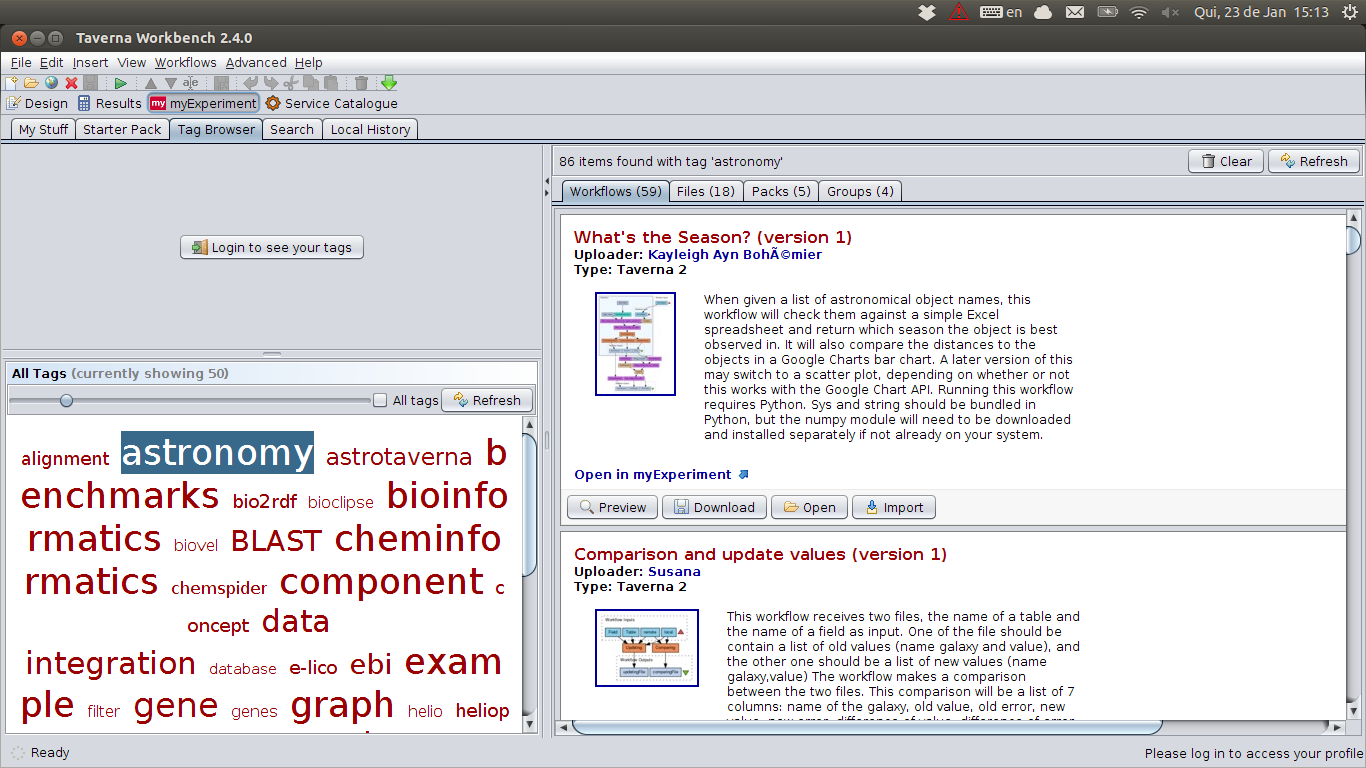
\includegraphics[width=1.1\textwidth]{img/taverna.png}
			\caption{Interface gráfica do Taverna}
		\end{figure}
		
		A linguagem Schfl possui uma serie de componentes que permite a representar no seu formato todo o workflow. A construção mais básica do Taverna são os \textit{Pipelines}, porém é possível criar construções de fluxos de dados como Agregação, Distribuição e Redistribuição de dados \cite{Teixeira2013}.
 	
 		Como pode ser visto na figura acima o Taverna possui uma integração com o \textit{myexperiment} para compartilhamento dos workflows modelados nele. O que talvez tenha o tornado um dos SGWC mais conhecidos, além de todo seu poder de construção de workflows científicos voltado para área Biológicas.
		
		\subsubsection{Pegasus}
		
		O SGWC Pegasus é um \textit{framework} que permite o mapeamento de instâncias de workflows em um conjuntos de recursos distribuídos, como uma grade. A descrição de um workflow no Pegasus é feita a partir de uma arquivo de entrada na forma de um DAG em formato XML, na linguagem DAX(\textit{Directed Acyclic Graph in XML}), que representa todo o fluxo de processamento e as dependências entre as tarefas, além dos recursos computacionais em que o workflow será executado\cite{Teixeira2013}.
		
		O DAX descreve os workflows termos de atividades, onde cada atividade consiste de um código de identificação da atividade, os nomes dos arquivos de entrada e saída de dados e uma relação de dependência entre as atividades. A partir dessa definição de dependências é possível construir as principais estruturas de fluxos de dados, \textit{pipelines}, distribuição, agregação e redistribuição de dados. O DAX também permite a definição de vários arquivos de saída que podem ser de tipos diferentes, dependo da necessidade da atividade\cite{Teixeira2013}. 
		
		 Código abaixo mostra como é representada uma atividade na linguagem DAX\footnote{https://confluence.pegasus.isi.edu/display/pegasus/WorkflowGenerator, Este exemplo foi retirado do DAX que representa o Montage}:
		

\begin{lstlisting}[language=XML, caption=Exemplo de uma atividade DAX]

<job id="ID000002" namespace="vahi" name="findrange" version="1.0" 
level="2"dv-namespace="vahi" dv-name="left"	dv-version="1.0">
	<argument>
		-a left -T 6 -i 
		<filename file="f.b1"/> -o <filename file="f.c1"/>
		-p 0.5
	</argument>
	<uses file="f.b1" link="input" dontRegister="false" dontTransfer="false" temporaryHint="true"/>
	<uses file="f.c1" link="output" dontRegister="true" dontTransfer="false" temporaryHint="true"/>
</job>

\end{lstlisting}

	Numa próxima fase o DAX é mapeado pelo Pegasus e as atividades definidas são executadas.
	
%colocar a definicao formal de redes de Petri, pegar na dissertacao da professra Kelly		OK
% se der tempo falar mais sobre redes de petri temporizadas e estocásticas
	\subsection{Redes de Petri}
		As Redes Petri(RdP) é um dos formalismos mais utilizados para modelagem analítica e análise de sistemas concorrentes mais utilizados,isso deve-se à fácil compreensão representação gráfica e devido ao seu potencial matemático para análise de modelos. Algumas características importantes de workflows científicos pôde ser facilmente representadas utilizando RdP, tais como a sincronização de tarefas, concorrência e controle de dependências\cite{Braghetto2011}.
		Uma RdP pode ser formalmente definida pela tupla $RdP={L,T,A,P,m_{0}}$, em que:
		\begin{itemize}
		\item $L=\{l_{1},l_{2},...,l_{L}\}$ é um conjunto de lugares;
		\item $T=\{t_{1},t_{2},...,t_{T}\}$ é um conjunto de transições;
		\item $A\subseteq(L x T)\bigcup (TxL)$ é um conjunto de arcos;
		\item $P: A \rightarrow \mathbbm{N}$ é a função peso dos arcos;
		\item $m_{0}=\{m_{01},m_{02},...,m_{0L}\}$ é a marcação inicial da rede;
		\end{itemize}
		
		Cada um dessas definições está associados a diferentes e importantes conceitos de RdP, que são:
		
			\begin{itemize}

				\item \textit{lugar} (representado graficamente por um círculo)- modela uma condição que deve ser satisfeita para que o disparo da transição seja realizado;

				\item \textit{transição} (representado graficamente por um retângulo) - pode ser compreendido por uma por uma acao ou um evento;

				\item \textit{arco orientado} liga um lugar a uma transição ou o contrário, ligando condições e eventos;

				\item \textit{fichas, marcas ou tokens} (representado por um ponto preto)- Representam um recurso ou um estado de um sistema;

				\item \textit{peso} - os arcos possuem um peso associado a eles; os pesos indica quantas fichas uma transição consome de um lugar de entrada ou quantas fichas uma transição acrescenta em um lugar de saída. Por \textit{default} quando um arco não possui um peso o peso é 1;
					
			\end{itemize}
			
			Da necessidade de modelagem de sistemas grandes e complexos, como os encontrados na natureza e na sociedade, foram definidas sobre a base de Redes de Petri clássica outras redes de alto nível, como as Redes de Petri Temporizadas(RdPTs) e Redes de Petri Estocásticas(RdPEs). As RdPTs como o nome diz permite modelar situações que ocorrem entre o início e fim de cada tarefa em termos do tempos. O permitiu diferentes possibilidades para modelagem, como lugares temporizados, fichas temporizadas e todas as outras estruturas descritas acima puderam ser tempodizadas e permitiram modelar uma série de sistemas reais. Já as RdPEs é uma subclasse das RdPTs, onde o tempo de atraso de uma transição é uma variável aleatória exponencialmente distribuída\cite{Braghetto2011}. 
		
	Ao se usar as redes de Petri para se modelar a execução de um workflow, cada vértice pode armazenar um ou mais tokens, os vértices de transição de redes de Petri podem consumir e produzir tokens de múltiplas localizações. Os vértices de transições agem em tokens de entrada por um processo denominado disparo. Quando uma transição é disparada, ela consome os tokens de suas posições de entrada, realiza alguma tarefa de processamento, e realoca um número específico de tokens nas suas posições de saída. Isso é feito atomicamente. Como os disparos são não-determinísticos, as redes de Petri são muito utilizadas para modelar comportamento concorrente em sistemas distribuídos. 	
			
		\subsubsection{PIPE}
			
			O PIPE\cite{PIPE} é uma ferramenta \textit{open source} criada para análise de RdPEs, possui uma interface gráfica simples e intuitiva. Com um conjunto de módulos para avaliar o comportamento estatístico das RdPEs, a representação de Lugares, Transições, Arcos e Fichas, segue o modelo gráfico descrito na seção anterior, como pode ser visto na figura abaixo:			
						
			\begin{figure}[h]
				\center
				\caption{Interface gráfica-PIPE}
				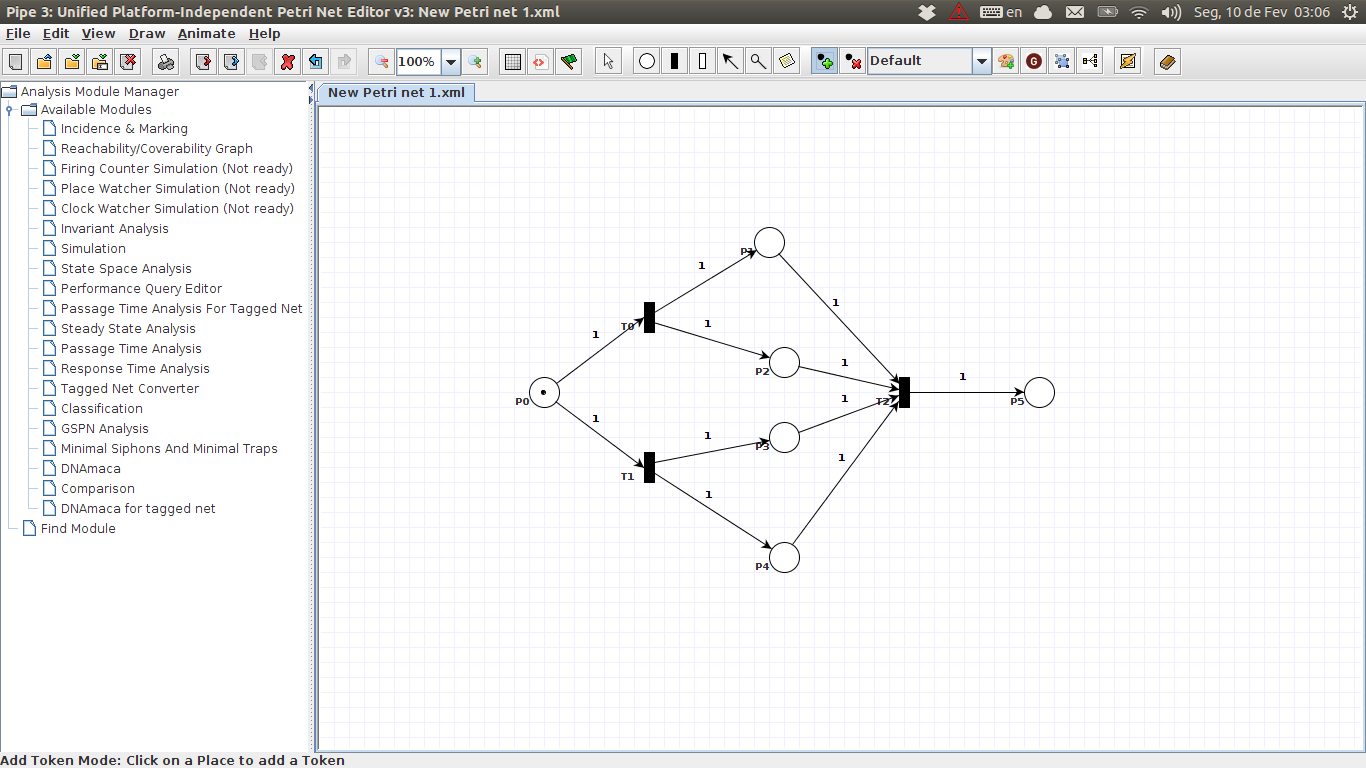
\includegraphics[width=1\textwidth]{img/pipe.jpg}
				\label{fig:PIPE}
			\end{figure}						
			
		Após a construção gráfica do modelo é possível observar a evolução dinâmica do sistema modelado e fazer a análise dos dados gerados, assim como exportar em formato XML ou o PNG da Rede Petri representada.
	%mostra como podemos aplicar redes de Petri na modelagem analitica de workflows cientificos
%relacionar modelage analítica de redes de Petri com workflows científicos	
%colocar porque escolhermos esse formalismo em vez de outros N/D
%colocar aqui como será modelado as redes de Petri para criar uma rede similar ao workflow analisado


	\subsection{Simuladores de workflows científicos}	
			
	Depois de criados os modelos em RdPEs para workflows científicos há algumas maneiras de validar o modelo, a primeira possibilidade é execução do workflows. Essa alternativa possui como problema o custo monetário envolvido na instanciação das máquinas, o que a torna inviável no primeiro momento. Uma outra alternativa mais viável é a  utilização de um ambiente de simulação computacional. Essa alternativa abre a possibilidade de criar-se diferentes ambientes computacionais e facilidade de reprodução da simulação, o que torna viável a busca por gargalos no workflows utilizados. Além da possibilidade de ter um avaliar modelos analíticos em um ambiente controlado que é um dos objetivos desse trabalho.
	
	Os simuladores possivelmente serão utilizados nesse trabalho estão brevemente descritos abaixo:
			\subsubsection{WorkflowSim}
	O WorkflowSim\cite{chen:workflowsim} é uma ferramenta de simulação de workflows científicos baseada no CloudSim\cite{google:cloudsim}, que também é uma ferramenta de simulação. No entanto, o CloudSim não possui certa características presentes no WorkflowSim, por exemplo, a simulação de ambientes heterogêneos e possibilidade de incluir falhas no sistema. As atividades no WorkflowSim  são descritas na linguagem DAX(XML gerado para execução de atividades no Pegasus). O WorkflowSim, possibilita também, modelar todo um ambiente computacional para execução dos workflows(Quantidade de \textit{Virtual Machine(VM)} e \textit{DataCenters}). Observe no Anexo 3 como é descrito um ambiente computacional no WorkflowSim. 
							
				
	%Para extrair índices de desempenho precisamos primeiro ter a solucao numerica do modelo, existem varias 				ferramentas para a modelagem de redes de Petri estocasticas e escolhemos utilizar a PIPE, ferramenta open source 		...
	% Para validar o índices de desempenho que serão extraidos na proxima fase do projeto, foram estudados alguns também 	simuladores, falar sobre o workflow_sim e cloud-sim_DVSF. No simulador é possível modelar o ambiente computacional 	e para avaliar a posteriore teremos que modelar esse ambiente computacional utilizando redes de Petri.
	%Falar sobre o DAX;caracterizar um workflow descrito por DAX e da possibilidade de converter um workflow em DAX em 	modelo analítico. Pegar um exemplo simples e colocar no relatório.
%Como foram realizadas as tarefas 

%Neste trabalho, a análise de desempenho de workflows científicos baseia-se em duas abordagens diferentes: primeiro, uma modelagem analítica, apoiando-se no formalismo estocástico de redes de Petri, segundo, a simulação dos workflows científicos no [CloudSim-DVSF]. Essas duas fases permitirá extrair e comparará-los.

% ---------------------------------------------------------------------------- %
%Metologia
% ---------------------------------------------------------------------------- %
\section{Metodologia}

	Nessa primeira fase do projeto foi realizado um estudo sobre os conceitos básicos envolvendo workflows, workflows científicos, Sistemas  Gerenciadores de Workflows Científicos(SGWC), Redes de Petri, ferramentas de representação de redes de Petri, modelagem analítica de workflows científicos(como o Montage) e Simuladores de workflows científicos. 
	%achar uma melhor forma para dizer essas coisas.
	Depois do estudo da bibliografia básica envolvendo workflow científicas e as motivações acadêmicas para a pesquisa de workflows científicas, foi feito o estudo de alguns SGWC, quanto a implementação de workflows e a representação do fluxo de dados em cada um deles.
	
	Para aparar o formalismo matemático evolvendo workflows científicos e fazer uma modelagem analítica de alguns workflows bem conhecidos foram estudas Redes de Petri, Redes de Petri Temporizadas e Redes de Petri Estocásticas, assim como uma ferramenta para representação gráfica e análise das RdPEs (PIPE).
	
	Para finalizar a primeira parte do trabalho foi feito um estudo do WorkFlowSim, quanto possibilidade de ferramenta de simulação para o projeto.
			
	%Depois do estudo de workflows científicos e suas características, para se extrair índices de desempenho dos workflows científicos e ter possibilidade de ser criar no futuro um algoritmo capaz de modelar analiticamente um workflow simples no forma DAX precisamos conhecer a estrutura de comportamento dos fluxo de dados dos workflows e caracterizar esse fluxo de dados extrair em alguns padrões de comportamento % colocar as possibilidades de fluxo de dados 
	%Assim modelamos em Redes de Petri um workflow bem conhecido pela conhecido pela comunidade o montagem como pode ser visto da figura abaixo:

	%Observe que apareceram algumas estruturas para modelar em Redes de Petri o Montage, isso mostra o poder dessa teoria em modelagem analítica de workflows científica, como foi visto acima com redes de Petri é possível criar sincronização, paralelismo...[Continuar depois]
	%Isso 
	
%A partido dos estudos... é possível automatizar a conversão de de modelos em DAX, sem grandes problemas.

% ---------------------------------------------------------------------------- %
%Resultados Parciais
% ---------------------------------------------------------------------------- %
\section{Resultados Parciais}
	
	Na primeira etapa desse projeto foram obtidos conhecimentos básico de workflows científicos, SGWC, RdPEs, modelagem analítica de workflow científicos. Para uma melhor interpretação foi feita a modelagem analítica do fluxo de dados do Montage, partir do Anexo 1, \cite{pegasus:workflowgenerator} com o auxilio PIPE. Como pode vista na figura do Anexo 2, que permitirá extrair índices de desempenho e verificar a validade do modelo a partir da simulação do Montage utilizando o WorkflowSim.



% ---------------------------------------------------------------------------- %
%Conclusões  Parciais
% ---------------------------------------------------------------------------- %
\section{Conclusões Parciais}
		
	 Todas as tarefas previstas no cronograma projeto foram realizadas com sucesso e estão listadas abaixo, assim como as atividades em andamento e as atividades futuras:

\subsection{Tarefas Realizadas}

	\begin{itemize}
			\item Estudo dos conceitos básicos relacionados a workflows científicos e seus respectivos modelos de representação de fluxo de dados;
			\item Estudo dos conceitos básicos relacionados à modelagem estocástica de workflows científicos;

			\item Identificação e caracterização do conjunto de construtores de fluxo de dados: Kepler, Taverna e Pegasus.
			\item Modelagem do Montage utilizando o PIPE;
			\item Estudo básido dos possíveis simuladores de workflows científicos para validar o modelo analítico criado.
	\end{itemize}

\subsection{Tarefas em Andamento}
		\begin{itemize}
		
			\item \textbf{2 meses} - Estudo da viabilidade do uso de diferentes tipos de formalismos estocásticos(em particular Redes de Petri e as Álgebra de processos estocásticos) para a modelagem de fluxos de dados;
			
			\item \textbf{15 dias} - Estudo do funcionamento do simuladores de workflows: WorkflowSim e Cloud-DVFS, quanto possibilidade de representação um ambiente computacional que possa ser modelado analiticamente;
		\end{itemize}

\subsection{Tarefas a serem realizadas}
		\begin{itemize}
			\item \textbf{15 dias}-Estudo e definição de índices extraídos a partir dos modelos representados na etapa anterior, que possam refletir um impacto no desempenho do fluxo de dados;
			\item \textbf{15 dias}- Montar uma simulação de workflow científico em um dos simuladores estudado na etapa anteriores;
			\item \textbf{1,5 meses}-Desenvolvimento de um algoritmo que faça a conversão automática de fluxo de dados de um fluxo de dados de workflow em um modelo estocástico correspondente(selecionado dentre os tipos de modelos estudados).
		\end{itemize}
 
\newpage
% ---------------------------------------------------------------------------- %
% Bibliografia
% ---------------------------------------------------------------------------- %
\bibliographystyle{apalike}% citação bibliográfica alpha
\bibliography{bibliografia}  % associado ao arquivo: 'bibliografia.bib'
%Colocar Figuras e cógigo nos anexos
\section{Anexos}
\subsection{Anexo 1}
	\begin{figure}[!h]
		\centering
		\caption{Ilustração do workflow do Montage}
			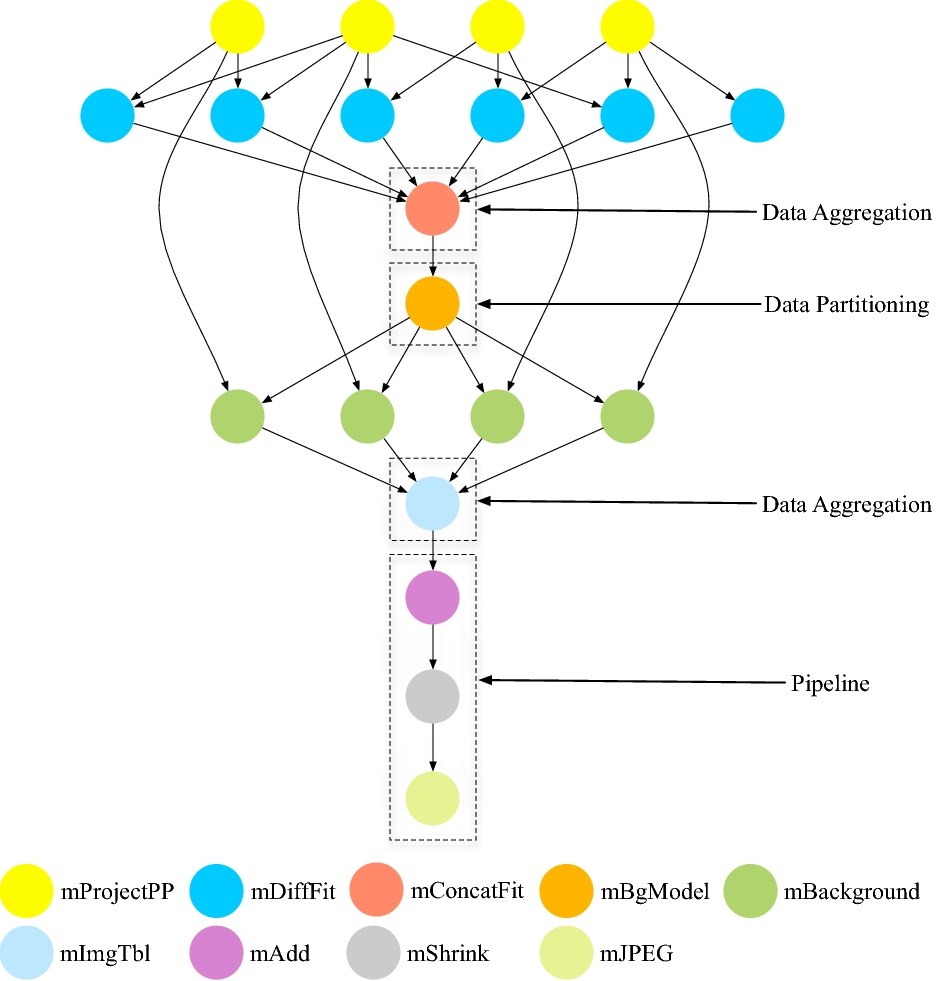
\includegraphics[width=1.1\textwidth]{img/Montage.jpg}
		\label{Anexo 1}
	\end{figure}



\subsection{Anexo 2}
\begin{landscape}
	\begin{figure}
		\centering
		\caption{Representação Gráfica do Montage usando Redes de Petri}
		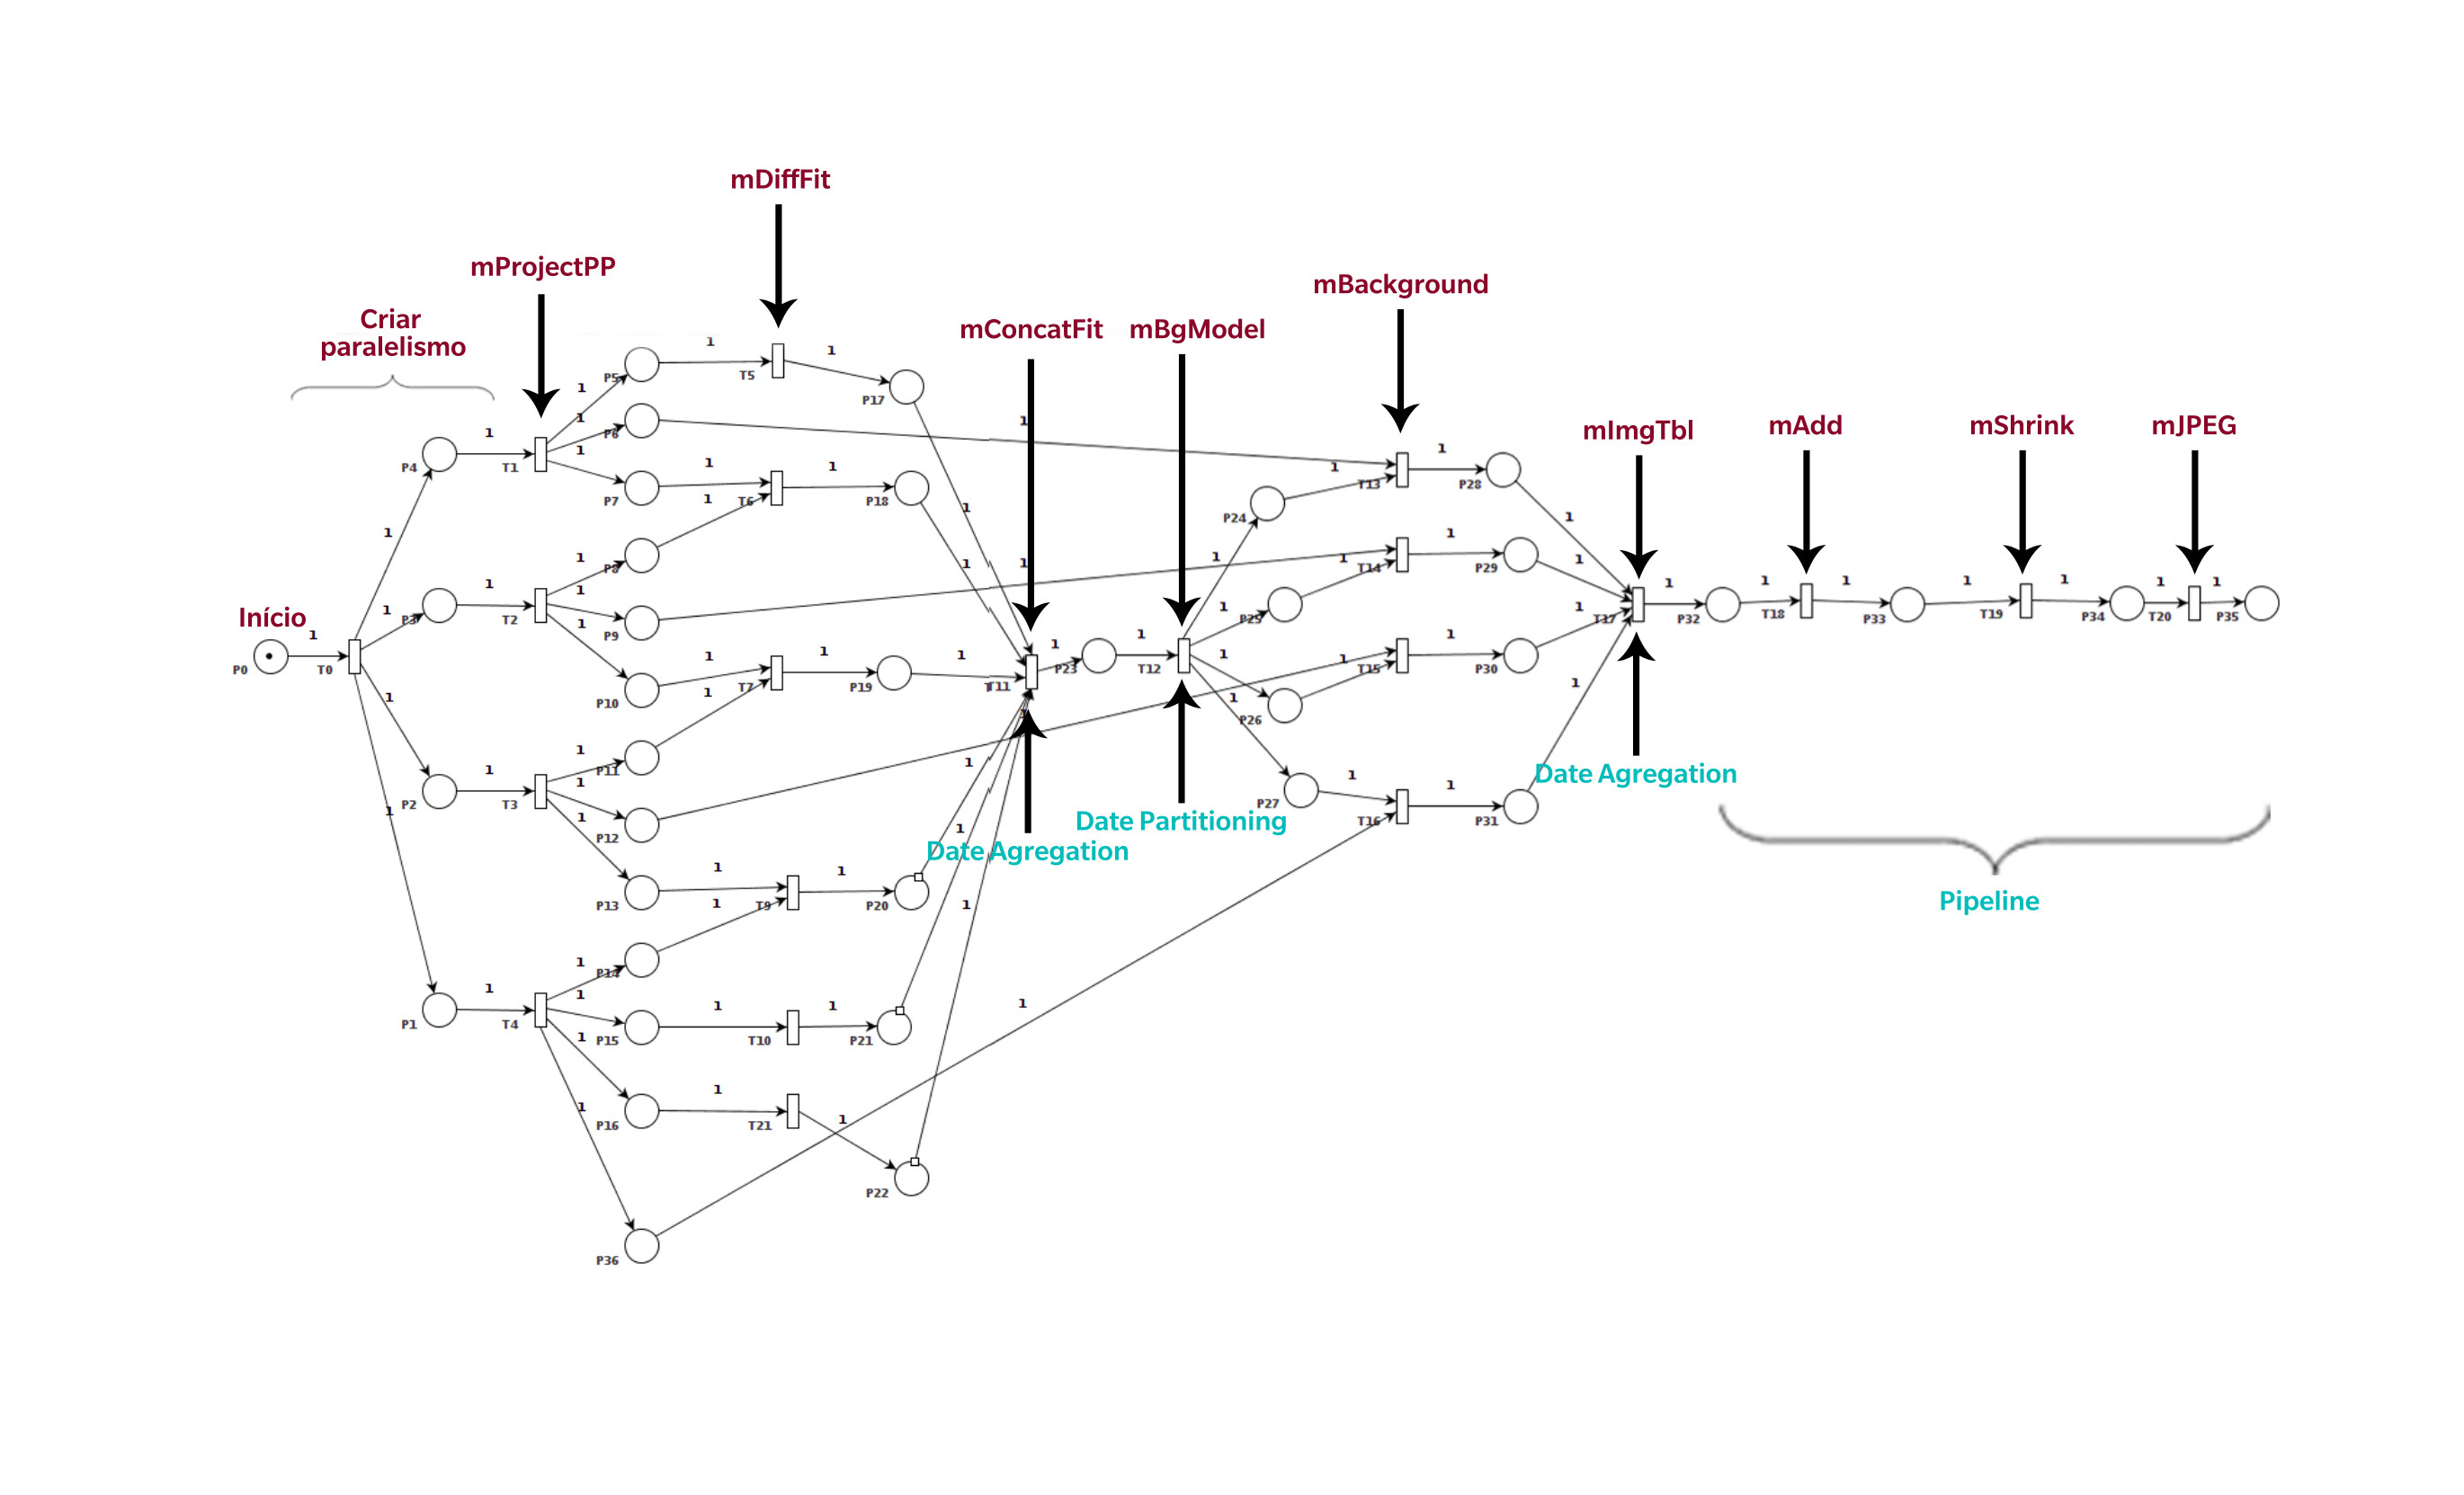
\includegraphics[width=2 \textwidth]{img/RP_montage.jpg}
		\label{Anexo 2}
	\end{figure}
\end{landscape}

\subsection{Anexo 3}
\begin{lstlisting}[caption=Descricão de uma ambiente computacional no WorkflowSim]

######Overhead Related Parameters
######The Workflow Engine Delay for level 1
#d1		= 8.1 
######The Workflow Engine Delay for level 2
#d2		= 18.44 
######The Workflow Engine Delay for other levels that are not specified 
#d0		= 6.74
######The Postscript Delay for level 1
#p1		= 78.05
######The Postscript Delay for level 2
#p2		= 13.12
######The Postscript Delay for other levels that are not specified
#p0		= 6.81
######The Queue Delay for level 1
#q1		= 77.75
######The Queue Delay for level 2
#q2		= 343.47
######The Queue Delay for other levels that are not specified
#q0		= 161.96
######The Clustering Delay for level 1
#c1		= 428.28
######The Clustering Delay for level 2
#c2		= 67.44
######The interval for Workflow Engine
#interval	= 5

######Failure related parameters
######The Task Failure Rate for level 1
#a1		= 0.02
######The Task Failure Rate for level 2
#a2		= 0.02
######Fault tolerant clustering method
#ftc.method	= FTCLUSTERING_DC
######Fault tolerant clustering monitor mode
#ftc.monitor	= MONITOR_ALL
######Fault tolerant clustering failure generation mode
#ftc.failure	= FAILURE_JOB

######Clustering Related parameters
######The number of clustered jobs per level
#clusters.num 	= 20
######The size of a clustered job (number of tasks per job)
#clusters.size 	= 20
######The clustering method
#clusters.method = horizontal
#clusters.method = balanced
######The type of file system to use
file.system	= LOCAL
#file.system	= SHARED

######Scheduling Related Parameters
######If you have specified planner.method, it will be disabled
scheduler.method= MINMIN_SCH

######Planning Related Parameters
#planner.method= RANDOM
#deadline = 100000

######Please replace it with your real physical path
dax.path = /home/duilio/workspace/WorkflowSim-1.0-master/config/dax/Montage_1000.xml
######Reducer mode used to remove duplicate dependencies
#reduce.method	= montage
\end{lstlisting}
\label{configworkflowsim}
\end{document}
